\documentclass[sigconf,nonacm]{acmart}

\usepackage{booktabs}
\usepackage{microtype}
\usepackage{tikz}
\usepackage{xcolor}
\usetikzlibrary{arrows.meta,positioning}

\settopmatter{printacmref=false,printfolios=true}
\renewcommand\footnotetextcopyrightpermission[1]{}
\pagestyle{plain}

\definecolor{benchgreen}{HTML}{005336}
\newcommand{\benchmarkname}{\textsc{PuzzleScript-World}}

\title{\benchmarkname: A Multi-Level Benchmark for Rule Learning,
Goal Recognition, and Planning}

\author{Adam Celermajer}
\affiliation{%
  \institution{Bar-Ilan University}
  \department{Department of Computer Science and Artificial Intelligence}
  \city{Ramat Gan}
  \country{Israel}
}
% Add supervisors or coauthors here once the author list is finalized.

\begin{document}

\begin{abstract}
Interactive agents entering a new environment must discover its dynamics,
recognize what constitutes success, and plan before this knowledge is complete.
A terminal success rate alone cannot determine which of these abilities
succeeded, nor whether knowledge acquired in one task was useful in the next.
We present \benchmarkname, a runnable benchmark environment built from
PuzzleScript games and exposed through an ARC-compatible interaction contract.
A single agent-driven action stream can be evaluated independently for
whole-game solving, pre-action goal recognition, and next-observation rule
inference. PuzzleScript's ordered levels make it possible to study a further
question that is largely hidden by collections of independent tasks:
cross-level transfer. The benchmark therefore specifies matched warm and cold
conditions while leaving agent memory control to the evaluator. The current
prototype includes a versioned 21-game public catalog, deterministic sampling,
optional rendered and symbolic observations, persisted scorecards, a live web
monitor, and replay-verified first-level solutions. We describe the benchmark
contract, scoring protocol, reference-solver status, and the experiments still
required to validate the benchmark empirically.
\end{abstract}

\keywords{interactive agents, benchmarks, PuzzleScript, rule learning,
goal recognition, planning, transfer learning}

\maketitle

\section{Introduction}

An agent acting in an unfamiliar environment faces several coupled problems.
It must identify the objects in its observations, infer how actions transform
them, discover the goal, and choose actions while its model remains uncertain.
Most interactive evaluations reduce this process to a terminal reward. This is
useful for measuring task completion, but it does not reveal whether a failure
came from an incorrect transition model, an incorrect goal hypothesis, or poor
planning.

PuzzleScript is a compact domain-specific language for authoring two-dimensional
puzzle games \cite{lavelle2013puzzlescript}. Its games provide hidden transition
rules, hidden win conditions, a small action space, and---most importantly---an
ordered sequence of levels. A later level may introduce a new object, generalize
a rule learned earlier, or combine familiar mechanics in a new way. A
PuzzleScript game is therefore not merely a collection of grids. It is a small
curriculum in which an agent can retain, revise, and reuse knowledge.

We introduce \benchmarkname, an environment for evaluating this process. The
agent queries the environment using an ARC-compatible contract, observes an
integer grid and optional representation aids, and submits actions until the
game is completed or its budget is exhausted. Before an action, the same agent
may optionally submit claims about the goal and the next transition. The
resulting real transition updates three separate score families:

\begin{itemize}
  \item \emph{game solving}: whether the ordered levels were completed and at
  what action cost;
  \item \emph{goal recognition}: whether the agent correctly predicted that
  its next action would complete the current level; and
  \item \emph{rule inference}: whether the agent correctly predicted the next
  observation, terminal state, and level change.
\end{itemize}

These scores are not collapsed into one headline number. They answer different
questions and can be enabled independently. The benchmark also exposes a
separate evaluator-only monitor so that game identity, reference data, and live
scores remain hidden from the agent.

The central research question is whether learning in earlier levels improves
later behavior. We formalize a matched comparison between a \emph{warm} agent
that reaches a target level sequentially and a \emph{cold} copy that begins
directly at that level. The environment provides matched tasks and scores; the
evaluator is responsible for preserving or clearing the external agent's
memory. This boundary keeps \benchmarkname{} an environment rather than an
agent orchestrator.

The present contribution is a benchmark design and working prototype, not yet
a completed agent comparison. The system currently provides a 21-game public
catalog, independent scorecards, a browser monitor, and replay-verified
reference trajectories. Controlled model comparisons, observation ablations,
and warm/cold transfer measurements remain future experimental work.

\section{Related Work}

\subsection{Interactive reasoning benchmarks}

ARC-AGI frames intelligence as skill-acquisition efficiency rather than
performance on a fixed task distribution \cite{chollet2019measure}. ARC-AGI-3
extends this direction to interactive environments in which an agent must
explore, model, set goals, and plan across a series of levels
\cite{arcprize2026arcagi3}. \benchmarkname{} adopts an ARC-compatible transport
surface so that an ARC-style agent can interact with either the local
PuzzleScript environment or another compatible backend. Its contribution is
the multi-level task substrate, separated diagnostic scores, and controlled
observation conditions rather than a new transport protocol.

\subsection{PuzzleScript environments}

PuzzleJAX compiles PuzzleScript-like programs into accelerated JAX transition
functions and demonstrates broad coverage across hundreds of games
\cite{earle2025puzzlejax}. This establishes PuzzleScript as a scalable source of
varied interactive environments. Our benchmark instead keeps the original
PuzzleScript engine as the authoritative runtime and targets rule learning,
goal recognition, sequential solving, and transfer between levels. Search
tools produce evaluator references; they are not the agent under evaluation.

\subsection{World-model evaluation}

WorldTest proposes evaluating learned world models through multiple global
environment queries, and AutumnBench instantiates the protocol with interactive
grid worlds and several query families \cite{warrier2026worldtest}. This
supports separating predictive knowledge from terminal return.
\benchmarkname{} similarly scores next-observation prediction independently of
solving, while adding hidden game goals, an explicit planning objective,
optional grounded representations, and ordered levels.

\section{Benchmark Environment}

\subsection{Games and interaction}

A game \(G\) is an ordered sequence of playable levels,
\[
G=(L_1,L_2,\ldots,L_m).
\]
A normal run starts at \(L_1\). Completing \(L_i\) advances the same session to
\(L_{i+1}\); non-playable message screens are excluded from the level count. At
step \(t\), the agent observes \(o_t\), selects a legal action \(a_t\), and
receives \(o_{t+1}\), a state label, and cumulative level progress. The hidden
rules and win conditions are executed by the original Node.js PuzzleScript
engine.

The mandatory observation is an ARC-style sequence of integer grids. A run may
also expose a rendered image, a ground-truth symbolic legend, and action
semantics. Each result records its representation condition. Grid-only,
rendered, and grounded symbolic runs are therefore comparable without treating
them as the same input.

\subsection{System architecture}

\begin{figure}[t]
  \centering
  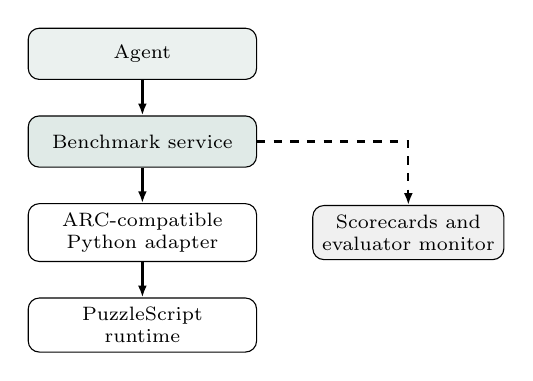
\begin{tikzpicture}[
    node distance=4.5mm,
    box/.style={draw, rounded corners, align=center, minimum height=6.5mm,
                minimum width=29mm, font=\scriptsize},
    arrow/.style={-{Latex[length=1.5mm]}, thick}
  ]
    \node[box, fill=benchgreen!8] (agent) {Agent};
    \node[box, below=of agent, fill=benchgreen!12] (bench)
      {Benchmark service};
    \node[box, below=of bench] (adapter)
      {ARC-compatible\\Python adapter};
    \node[box, below=of adapter] (runtime)
      {PuzzleScript\\runtime};
    \node[box, right=7mm of adapter, fill=gray!12,
          minimum width=24mm] (monitor)
      {Scorecards and\\evaluator monitor};

    \draw[arrow] (agent) -- (bench);
    \draw[arrow] (bench) -- (adapter);
    \draw[arrow] (adapter) -- (runtime);
    \draw[arrow, dashed] (bench.east) -| (monitor.north);
  \end{tikzpicture}
  \caption{The agent calls the environment. Each authoritative transition is
  executed once and can update every enabled score. Ground truth and monitoring
  are available only to the evaluator.}
  \label{fig:architecture}
\end{figure}

The split runtime follows from the implementation: the PuzzleScript engine is
distributed as an npm package, so a Node.js service wraps game execution. A
Python service adapts that runtime to the public ARC interaction contract. The
benchmark layer adds catalog sampling, opaque aliases, observation filtering,
claims, scoring, persistence, and monitoring.

The benchmark does not require an \texttt{agent\_url}. The direction of control
is agent-to-environment: an external client opens a run and submits actions.
This follows the normal environment interface and avoids requiring the
benchmark to launch, restart, or inspect arbitrary agents.

\subsection{Run protocol}

A run is defined by a benchmark version, sampled game identifiers, a random
seed, action budgets, enabled score families, and an observation condition.
The agent receives an opaque game identifier and a session credential.
Evaluator credentials are separate. At every step:

\begin{enumerate}
  \item the agent receives the current observation and legal actions;
  \item it may attach a goal claim and a next-transition prediction;
  \item it submits exactly one action;
  \item the runtime executes that action; and
  \item the environment updates progress and every enabled score.
\end{enumerate}

This protocol lets one run measure multiple abilities without generating
different trajectories for each scorer. Missing optional claims affect the
coverage of the relevant score but do not prevent the agent from acting.

\section{Scoring}

\subsection{Game solving}

Let \(c_g\) be the number of completed playable levels and \(m_g\) the total
number of playable levels. The diagnostic completion rate is
\[
C_g=\frac{c_g}{m_g},
\]
and the primary solving score is binary whole-game completion,
\[
S_g=\mathbb{I}[c_g=m_g].
\]
This definition prevents a game with many easy introductory levels from
appearing solved when its later levels remain incomplete.

When a replay-verified whole-game reference has \(A_g^\star\) actions and the
agent solves the game in \(A_g\) actions, action efficiency is
\[
E_g=\min\left(1,\frac{A_g^\star}{A_g}\right).
\]
Efficiency is omitted if the agent does not solve the game or no whole-game
reference exists. A replay-valid path is an upper bound on solution length
unless shortest-path optimality has been proved separately.

\subsection{Goal recognition}

Before each action, the agent may predict a probability \(p_t\) that the action
will complete the current level. The transition supplies the binary label
\(y_t\). The scorecard reports balanced accuracy, F1, coverage, and the Brier
score,
\[
\operatorname{Brier}=\frac{1}{T}\sum_{t=1}^{T}(p_t-y_t)^2.
\]
Claims must be submitted before the outcome is observed. Missing claims lower
coverage and count as incorrect in the primary classification denominator.
This operational target is narrower than asking an evaluator to grade a
free-form natural-language goal description, but it is reproducible and can be
scored online.

\subsection{Rule inference}

Before acting, the agent may predict the next integer grid, terminal state, and
level delta. The real transition is then the ground truth. Diagnostics include
exact-transition accuracy, exact-frame accuracy, cell accuracy, changed-cell
F1, state accuracy, level-delta accuracy, and coverage. This tests whether the
agent's learned rules have executable predictive content rather than whether a
natural-language explanation sounds plausible.

\subsection{Cross-level transfer}

For a target level \(L_k\), the evaluator may create two matched runs:

\begin{itemize}
  \item a \emph{warm} run that begins at \(L_1\) and reaches \(L_k\)
  sequentially while the evaluator retains agent memory; and
  \item a \emph{cold} run that begins directly at \(L_k\) with a fresh copy of
  the same agent and the same representation and target-level budget.
\end{itemize}

The environment scores the two conditions independently. If both solve the
target level in \(A_k^{\mathrm{warm}}\) and \(A_k^{\mathrm{cold}}\) actions, a
descriptive transfer gain is
\[
T_k=
\frac{A_k^{\mathrm{cold}}-A_k^{\mathrm{warm}}}
     {A_k^{\mathrm{cold}}}.
\]
Raw completion and action counts remain primary because this ratio is not
meaningful when either condition fails. Results must state
\texttt{memory\_reset=user\_managed}: an environment cannot prove that an
external agent cleared files, caches, model state, or other memory.

\section{Prototype Status}

\subsection{Implemented environment}

The current public manifest identifies benchmark version 0.3.0. The prototype
provides:

\begin{itemize}
  \item agent-initiated runs over an ARC-compatible REST contract;
  \item deterministic catalog sampling by seed;
  \item separate agent and evaluator-monitor credentials;
  \item optional rendered images, legends, and action semantics;
  \item independent solving, goal-recognition, and rule-inference scorecards;
  \item persisted run envelopes and a browser-based live monitor; and
  \item a deliberately simple baseline client that exercises the contract.
\end{itemize}

\subsection{Catalog and replay references}

The checked-in public catalog contains 21 games. Every catalog entry has a
replay-verified winning trajectory for its selected first playable level. An
initial bounded breadth-first search attempted 30 sampled first playable levels
and solved 21 within its state or time limits. A later targeted solver produced
valid winning paths for the remaining nine first-level cases. Table
\ref{tab:targeted} reports their replay-verified action counts. These counts are
valid upper bounds unless exact optimality is established separately.

\begin{table}[t]
  \caption{Previously unresolved first-level references.}
  \label{tab:targeted}
  \centering
  \small
  \begin{tabular}{lrr}
    \toprule
    Game & Level & Actions \\
    \midrule
    Fire in Winter     & 2 & 65 \\
    Self Alteration    & 2 & 22 \\
    Collapsing Tiles   & 2 & 14 \\
    Fuse to Green      & 2 & 19 \\
    Dark Pellets       & 3 & 21 \\
    Infected           & 2 & 27 \\
    Extra Push         & 2 & 42 \\
    The Art of Storage & 2 & 51 \\
    Side Painting      & 3 & 34 \\
    \midrule
    Total              &   & 295 \\
    \bottomrule
  \end{tabular}
\end{table}

Together, the search artifacts contain first-level winning trajectories for all
30 sampled games. The public benchmark remains the checked-in 21-game subset;
suite expansion and freezing are part of the planned work.

\subsection{Whole-game reference}

The prototype whole-game solver filters message screens, solves playable
levels sequentially, preserves cumulative progress, and validates the final
action stream in the authoritative engine. For
\texttt{ps\_sokoban\_basic-v1}, it replay-verified both playable levels at
depths 33 and 16, for 49 actions in total. This is currently the only catalog
game with a complete whole-game reference. Consequently, action-efficiency
results for other games are intentionally not reported.

\section{Planned Evaluation}

The empirical evaluation will answer four questions:

\begin{description}
  \item[RQ1: Solving.] Which agents complete entire ordered games under fixed
  action and compute budgets?
  \item[RQ2: Diagnosis.] Do the goal-recognition and rule-inference scores
  distinguish failures that have similar terminal returns?
  \item[RQ3: Transfer.] Does experience in earlier levels improve target-level
  completion or action cost relative to a matched cold start?
  \item[RQ4: Representation.] How do anonymous grids, rendered observations,
  symbolic legends, and action semantics affect each score family?
\end{description}

The suite will first be frozen with versioned games, seeds, budgets, observation
conditions, score aggregation, and failure policy. We will then evaluate the
baseline client and selected learning agents. Results will report per-game
whole-game completion, per-level progress, action counts, efficiency where a
reference exists, goal-recognition metrics, rule-inference metrics, token use,
and cost.

Warm/cold comparisons will use identical target levels, observations, and
budgets. The warm condition will retain agent state across preceding levels;
the cold condition will use a fresh external process. Later levels will be
annotated by whether they introduce an object or mechanic, generalize an
existing rule, or produce a new interaction among known rules. This supports
analysis of positive transfer, negative transfer, and belief revision.

\begin{table}[t]
  \caption{Current evidence and intentionally unreported results.}
  \label{tab:status}
  \centering
  \small
  \begin{tabular}{p{0.43\columnwidth}p{0.47\columnwidth}}
    \toprule
    Available now & Not yet measured \\
    \midrule
    Runnable environment and baseline client &
    Controlled comparison of learning agents \\
    Independent online scorecards &
    Warm/cold cross-level transfer \\
    21-game public catalog &
    Grid/image/legend ablation \\
    30 first-level winning replays &
    Whole-game references beyond Sokoban \\
    One 49-action whole-game replay &
    Statistical confidence intervals \\
    \bottomrule
  \end{tabular}
\end{table}

\section{Limitations}

Reference search has access to game files and therefore measures environment
structure, not an agent's ability to learn unknown rules. A shortest execution
path under known rules is also not an optimal learning policy: defining the
latter would require a hypothesis space, prior, and exploration-cost objective.
The benchmark therefore uses references only for solving efficiency.

The current goal-recognition target asks whether the next action completes a
level. It is objective and online, but does not capture every useful form of
goal representation. Likewise, next-frame prediction tests operational
transition knowledge without proving that the agent formed a compact or
causally correct rule set.

Finally, external memory control is outside the environment boundary. Warm/cold
transfer results depend on evaluator discipline and must disclose the reset
procedure. These limitations are explicit parts of the reporting contract
rather than hidden assumptions.

\section{Conclusion}

\benchmarkname{} turns PuzzleScript's ordered games into an interactive
evaluation surface for solving, goal recognition, rule inference, and
cross-level transfer. Its central design choice is to preserve one
authoritative action stream while reporting each ability separately. The
prototype establishes that the environment, scorecards, monitoring surface,
and replay pipeline are runnable. The remaining work is empirical: complete
whole-game references, freeze the suite, compare agents and representations,
and test whether knowledge acquired in early levels produces measurable gains
later in the same game.

\bibliographystyle{ACM-Reference-Format}
\bibliography{proposalbib}

\end{document}
